\documentclass[]{article}
\usepackage{lmodern}
\usepackage{amssymb,amsmath}
\usepackage{ifxetex,ifluatex}
\usepackage{fixltx2e} % provides \textsubscript
\ifnum 0\ifxetex 1\fi\ifluatex 1\fi=0 % if pdftex
  \usepackage[T1]{fontenc}
  \usepackage[utf8]{inputenc}
\else % if luatex or xelatex
  \ifxetex
    \usepackage{mathspec}
  \else
    \usepackage{fontspec}
  \fi
  \defaultfontfeatures{Ligatures=TeX,Scale=MatchLowercase}
\fi
% use upquote if available, for straight quotes in verbatim environments
\IfFileExists{upquote.sty}{\usepackage{upquote}}{}
% use microtype if available
\IfFileExists{microtype.sty}{%
\usepackage{microtype}
\UseMicrotypeSet[protrusion]{basicmath} % disable protrusion for tt fonts
}{}
\usepackage[margin=1in]{geometry}
\usepackage{hyperref}
\hypersetup{unicode=true,
            pdftitle={Graphical Simulation of Tissue microarray (TMA)},
            pdfborder={0 0 0},
            breaklinks=true}
\urlstyle{same}  % don't use monospace font for urls
\usepackage{color}
\usepackage{fancyvrb}
\newcommand{\VerbBar}{|}
\newcommand{\VERB}{\Verb[commandchars=\\\{\}]}
\DefineVerbatimEnvironment{Highlighting}{Verbatim}{commandchars=\\\{\}}
% Add ',fontsize=\small' for more characters per line
\usepackage{framed}
\definecolor{shadecolor}{RGB}{248,248,248}
\newenvironment{Shaded}{\begin{snugshade}}{\end{snugshade}}
\newcommand{\AlertTok}[1]{\textcolor[rgb]{0.94,0.16,0.16}{#1}}
\newcommand{\AnnotationTok}[1]{\textcolor[rgb]{0.56,0.35,0.01}{\textbf{\textit{#1}}}}
\newcommand{\AttributeTok}[1]{\textcolor[rgb]{0.77,0.63,0.00}{#1}}
\newcommand{\BaseNTok}[1]{\textcolor[rgb]{0.00,0.00,0.81}{#1}}
\newcommand{\BuiltInTok}[1]{#1}
\newcommand{\CharTok}[1]{\textcolor[rgb]{0.31,0.60,0.02}{#1}}
\newcommand{\CommentTok}[1]{\textcolor[rgb]{0.56,0.35,0.01}{\textit{#1}}}
\newcommand{\CommentVarTok}[1]{\textcolor[rgb]{0.56,0.35,0.01}{\textbf{\textit{#1}}}}
\newcommand{\ConstantTok}[1]{\textcolor[rgb]{0.00,0.00,0.00}{#1}}
\newcommand{\ControlFlowTok}[1]{\textcolor[rgb]{0.13,0.29,0.53}{\textbf{#1}}}
\newcommand{\DataTypeTok}[1]{\textcolor[rgb]{0.13,0.29,0.53}{#1}}
\newcommand{\DecValTok}[1]{\textcolor[rgb]{0.00,0.00,0.81}{#1}}
\newcommand{\DocumentationTok}[1]{\textcolor[rgb]{0.56,0.35,0.01}{\textbf{\textit{#1}}}}
\newcommand{\ErrorTok}[1]{\textcolor[rgb]{0.64,0.00,0.00}{\textbf{#1}}}
\newcommand{\ExtensionTok}[1]{#1}
\newcommand{\FloatTok}[1]{\textcolor[rgb]{0.00,0.00,0.81}{#1}}
\newcommand{\FunctionTok}[1]{\textcolor[rgb]{0.00,0.00,0.00}{#1}}
\newcommand{\ImportTok}[1]{#1}
\newcommand{\InformationTok}[1]{\textcolor[rgb]{0.56,0.35,0.01}{\textbf{\textit{#1}}}}
\newcommand{\KeywordTok}[1]{\textcolor[rgb]{0.13,0.29,0.53}{\textbf{#1}}}
\newcommand{\NormalTok}[1]{#1}
\newcommand{\OperatorTok}[1]{\textcolor[rgb]{0.81,0.36,0.00}{\textbf{#1}}}
\newcommand{\OtherTok}[1]{\textcolor[rgb]{0.56,0.35,0.01}{#1}}
\newcommand{\PreprocessorTok}[1]{\textcolor[rgb]{0.56,0.35,0.01}{\textit{#1}}}
\newcommand{\RegionMarkerTok}[1]{#1}
\newcommand{\SpecialCharTok}[1]{\textcolor[rgb]{0.00,0.00,0.00}{#1}}
\newcommand{\SpecialStringTok}[1]{\textcolor[rgb]{0.31,0.60,0.02}{#1}}
\newcommand{\StringTok}[1]{\textcolor[rgb]{0.31,0.60,0.02}{#1}}
\newcommand{\VariableTok}[1]{\textcolor[rgb]{0.00,0.00,0.00}{#1}}
\newcommand{\VerbatimStringTok}[1]{\textcolor[rgb]{0.31,0.60,0.02}{#1}}
\newcommand{\WarningTok}[1]{\textcolor[rgb]{0.56,0.35,0.01}{\textbf{\textit{#1}}}}
\usepackage{graphicx,grffile}
\makeatletter
\def\maxwidth{\ifdim\Gin@nat@width>\linewidth\linewidth\else\Gin@nat@width\fi}
\def\maxheight{\ifdim\Gin@nat@height>\textheight\textheight\else\Gin@nat@height\fi}
\makeatother
% Scale images if necessary, so that they will not overflow the page
% margins by default, and it is still possible to overwrite the defaults
% using explicit options in \includegraphics[width, height, ...]{}
\setkeys{Gin}{width=\maxwidth,height=\maxheight,keepaspectratio}
\IfFileExists{parskip.sty}{%
\usepackage{parskip}
}{% else
\setlength{\parindent}{0pt}
\setlength{\parskip}{6pt plus 2pt minus 1pt}
}
\setlength{\emergencystretch}{3em}  % prevent overfull lines
\providecommand{\tightlist}{%
  \setlength{\itemsep}{0pt}\setlength{\parskip}{0pt}}
\setcounter{secnumdepth}{0}
% Redefines (sub)paragraphs to behave more like sections
\ifx\paragraph\undefined\else
\let\oldparagraph\paragraph
\renewcommand{\paragraph}[1]{\oldparagraph{#1}\mbox{}}
\fi
\ifx\subparagraph\undefined\else
\let\oldsubparagraph\subparagraph
\renewcommand{\subparagraph}[1]{\oldsubparagraph{#1}\mbox{}}
\fi

%%% Use protect on footnotes to avoid problems with footnotes in titles
\let\rmarkdownfootnote\footnote%
\def\footnote{\protect\rmarkdownfootnote}

%%% Change title format to be more compact
\usepackage{titling}

% Create subtitle command for use in maketitle
\newcommand{\subtitle}[1]{
  \posttitle{
    \begin{center}\large#1\end{center}
    }
}

\setlength{\droptitle}{-2em}
  \title{Graphical Simulation of Tissue microarray (TMA)}
  \pretitle{\vspace{\droptitle}\centering\huge}
  \posttitle{\par}
  \author{}
  \preauthor{}\postauthor{}
  \predate{\centering\large\emph}
  \postdate{\par}
  \date{2018-01-14}


\begin{document}
\maketitle

\hypertarget{what-is-tissue-microarray-tma}{%
\section{What is Tissue microarray
(TMA)}\label{what-is-tissue-microarray-tma}}

In oncology, identifying biomarker is clinically relevant. Biomarker
here refers to

\begin{quote}
``any measurement reflecting an interaction between a biological system
and a potential hazard\ldots{} (and the) measured response may be
functional and physiological, biochemical at the cellular level, or a
molecular interaction.''\footnote{\href{http://www.inchem.org/documents/ehc/ehc/ehc155.htm}{WHO
  International Programme on Chemical Safety Biomarkers and Risk
  Assessment}}
\end{quote}

Tissue microarray is a set of slides contain ``many small representative
tissue samples from hundreds of different cases assembled on a single
histologic slide'' \footnote{\href{https://www.ncbi.nlm.nih.gov/pmc/articles/PMC2813639/}{Tissue
  Microarray: A rapidly evolving diagnostic and research tool}}. Each
sample spot is well-annotated with various clinical and pathological
information from the patient of origin. TMA can be regarded as a high
throughput method (in contrast to common tissue staining with one tissue
per slide) in effectively establishing disease association to molecular
expression.

To quantify the expression of molecule, immunohistochemstry (IHC) is one
of the common method to visualise the protein quantity: the more target
contains, the more brownish it stains. The brownish color is due to the
use of Diammonium phosphate (DAP) that is able to conjugate with the
antibodies. The brownish-free region usually is usually blue due to the
Hematoxylin counter stain that target to nuclei.

\href{/tma.jpg}{a typical TMA slide with array of tissue spots}

Although there are various algorithms and software that automate
quantification process, manual quantification staining intensity is
still commonly used. Manual scoring produces a score which is a
consensus of at least two independent pathologists.

The first step of scoring involve identification the total percentage of
yellow area within the area/compartment of interest (e.g.~cytoplasm of
the tumor cell); then the total percentage will be split into 3
categories of intensity.

\hypertarget{building-a-ihc-reference-image-with-5-increment-in-total-percentage-of-dap-staining}{%
\section{Building a IHC reference image with 5\% increment in total
percentage of DAP
staining}\label{building-a-ihc-reference-image-with-5-increment-in-total-percentage-of-dap-staining}}

Each TMA spot is a round patch of color; so a group of evenly
distributed
\href{https://stackoverflow.com/questions/5837572/generate-a-random-point-within-a-circle-uniformly/5838055\#5838055}{points
within the circle is generated}. There is a 30\% of none stained area,
which is represented by 30\% dot are color as white (\#FFFFFF), the
color of background. The rest 70\% stained area is further divided into
DAP stain (brown stain as \#AA6845\footnote{Hexcode from Digital Color
  \href{mailto:Meter@Mac}{\nolinkurl{Meter@Mac}} with Display in sRGB
  setting}) and

\begin{Shaded}
\begin{Highlighting}[]
\NormalTok{x <-}\StringTok{ }\KeywordTok{c}\NormalTok{(}\StringTok{"tidyverse"}\NormalTok{, }\StringTok{"gridExtra"}\NormalTok{)}
\KeywordTok{lapply}\NormalTok{(x, require, }\DataTypeTok{character.only =} \OtherTok{TRUE}\NormalTok{, }\DataTypeTok{quietly =}\NormalTok{ T,  }\DataTypeTok{warn.conflicts =}\NormalTok{ F)}
\end{Highlighting}
\end{Shaded}

\begin{verbatim}
## -- Attaching packages -------------------------------- tidyverse 1.2.1 --
\end{verbatim}

\begin{verbatim}
## √ ggplot2 2.2.1     √ purrr   0.2.4
## √ tibble  1.4.2     √ dplyr   0.7.4
## √ tidyr   0.8.0     √ stringr 1.3.0
## √ readr   1.1.1     √ forcats 0.3.0
\end{verbatim}

\begin{verbatim}
## -- Conflicts ----------------------------------- tidyverse_conflicts() --
## x dplyr::filter() masks stats::filter()
## x dplyr::lag()    masks stats::lag()
\end{verbatim}

\begin{verbatim}
## [[1]]
## [1] TRUE
## 
## [[2]]
## [1] TRUE
\end{verbatim}

\begin{Shaded}
\begin{Highlighting}[]
\NormalTok{perc_plot <-}\StringTok{ }\ControlFlowTok{function}\NormalTok{(}\DataTypeTok{B =} \DecValTok{10000}\NormalTok{, freq, }\DataTypeTok{nonstain_freq =} \FloatTok{.3}\NormalTok{, }\DataTypeTok{bg =} \StringTok{"#FFFFFF"}\NormalTok{, }\DataTypeTok{DAP =} \StringTok{"#AA6845"}\NormalTok{, }\DataTypeTok{hematoxylin =} \StringTok{"#38A5D3"}\NormalTok{)\{}
\NormalTok{    t <-}\StringTok{ }\DecValTok{2}\OperatorTok{*}\NormalTok{pi}\OperatorTok{*}\KeywordTok{runif}\NormalTok{(}\DataTypeTok{n =}\NormalTok{ B)}
\NormalTok{    u <-}\StringTok{ }\KeywordTok{runif}\NormalTok{(}\DataTypeTok{n =}\NormalTok{ B) }\OperatorTok{+}\StringTok{ }\KeywordTok{runif}\NormalTok{(}\DataTypeTok{n =}\NormalTok{ B)}

\NormalTok{    r <-}\StringTok{ }\KeywordTok{sapply}\NormalTok{(u, }\ControlFlowTok{function}\NormalTok{(i) \{}
        \ControlFlowTok{if}\NormalTok{ (i}\OperatorTok{>}\DecValTok{1}\NormalTok{) \{}
            \DecValTok{2}\OperatorTok{-}\NormalTok{i }
\NormalTok{        \} }\ControlFlowTok{else}\NormalTok{ \{}
\NormalTok{            i}
\NormalTok{        \}\})}
    
\NormalTok{    r <-}\StringTok{ }\KeywordTok{tbl_df}\NormalTok{(}\KeywordTok{matrix}\NormalTok{(r, }\DataTypeTok{ncol =} \DecValTok{1}\NormalTok{))}

\NormalTok{    samp_rdm <-}\StringTok{ }\KeywordTok{sample}\NormalTok{(}\KeywordTok{c}\NormalTok{(}\KeywordTok{rep.int}\NormalTok{(}\DecValTok{0}\NormalTok{, B}\OperatorTok{*}\NormalTok{nonstain_freq), }\KeywordTok{rep.int}\NormalTok{(}\DecValTok{1}\NormalTok{, B}\OperatorTok{*}\NormalTok{(}\DecValTok{1}\OperatorTok{-}\NormalTok{nonstain_freq)}\OperatorTok{*}\NormalTok{freq}\OperatorTok{+}\DecValTok{1}\NormalTok{), }\KeywordTok{rep.int}\NormalTok{(}\DecValTok{2}\NormalTok{, B}\OperatorTok{*}\NormalTok{(}\DecValTok{1}\OperatorTok{-}\NormalTok{nonstain_freq)}\OperatorTok{*}\NormalTok{(}\DecValTok{1}\OperatorTok{-}\NormalTok{freq)}\OperatorTok{+}\DecValTok{1}\NormalTok{)), }\DataTypeTok{size =}\NormalTok{ B) }
\NormalTok{    ## use ~rep.int~ instread of ~rep~, since the danger of having argument time as an operation. see help("rep")}
    
\NormalTok{    r }\OperatorTok
\StringTok{        }\KeywordTok{mutate}\NormalTok{(., }\DataTypeTok{x =}\NormalTok{  .[[}\DecValTok{1}\NormalTok{]]}\OperatorTok{*}\KeywordTok{cos}\NormalTok{(t), }\DataTypeTok{y =}\NormalTok{  .[[}\DecValTok{1}\NormalTok{]]}\OperatorTok{*}\KeywordTok{sin}\NormalTok{(t), }\DataTypeTok{stained =} \KeywordTok{factor}\NormalTok{(samp_rdm)) }\OperatorTok
\StringTok{        }\KeywordTok{ggplot}\NormalTok{(}\KeywordTok{aes}\NormalTok{(}\DataTypeTok{x =}\NormalTok{ x, }\DataTypeTok{y =}\NormalTok{ y, }\DataTypeTok{color =}\NormalTok{ stained)) }\OperatorTok{+}\StringTok{ }\KeywordTok{geom_point}\NormalTok{()}\OperatorTok{+}\KeywordTok{coord_fixed}\NormalTok{()}\OperatorTok{+}
\StringTok{        }\KeywordTok{scale_color_manual}\NormalTok{(}\DataTypeTok{values =} \KeywordTok{c}\NormalTok{(bg, DAP, hematoxylin)) }\OperatorTok{+}
\StringTok{        }\KeywordTok{labs}\NormalTok{(}\DataTypeTok{subtitle=} \KeywordTok{paste0}\NormalTok{(freq}\OperatorTok{*}\DecValTok{100}\NormalTok{, }\StringTok{"% DAP staining"}\NormalTok{))}\OperatorTok{+}
\StringTok{        }\KeywordTok{theme}\NormalTok{(}\DataTypeTok{axis.line=}\KeywordTok{element_blank}\NormalTok{(),}
              \DataTypeTok{plot.subtitle =} \KeywordTok{element_text}\NormalTok{(}\DataTypeTok{size=}\DecValTok{35}\NormalTok{),}
              \DataTypeTok{axis.text.x=}\KeywordTok{element_blank}\NormalTok{(),}
              \DataTypeTok{axis.text.y=}\KeywordTok{element_blank}\NormalTok{(),}
              \DataTypeTok{axis.ticks=}\KeywordTok{element_blank}\NormalTok{(),}
              \DataTypeTok{axis.title.x=}\KeywordTok{element_blank}\NormalTok{(),}
              \DataTypeTok{axis.title.y=}\KeywordTok{element_blank}\NormalTok{(),}
              \DataTypeTok{legend.position=}\StringTok{"none"}\NormalTok{,}
              \DataTypeTok{panel.background=}\KeywordTok{element_blank}\NormalTok{(),}
              \DataTypeTok{panel.border=}\KeywordTok{element_blank}\NormalTok{(),}
              \DataTypeTok{panel.grid.major=}\KeywordTok{element_blank}\NormalTok{(),}
              \DataTypeTok{panel.grid.minor=}\KeywordTok{element_blank}\NormalTok{(),}
              \DataTypeTok{plot.background=}\KeywordTok{element_blank}\NormalTok{())}
\NormalTok{\}}


\NormalTok{tp <-}\StringTok{ }\KeywordTok{lapply}\NormalTok{(}\KeywordTok{seq}\NormalTok{(}\DataTypeTok{from =} \FloatTok{0.05}\NormalTok{, }\DataTypeTok{to =} \DecValTok{1}\NormalTok{, }\DataTypeTok{by =} \FloatTok{0.05}\NormalTok{), }\ControlFlowTok{function}\NormalTok{(n) }\KeywordTok{perc_plot}\NormalTok{(}\DataTypeTok{freq =}\NormalTok{ n))}


\KeywordTok{do.call}\NormalTok{(grid.arrange,tp)}
\end{Highlighting}
\end{Shaded}

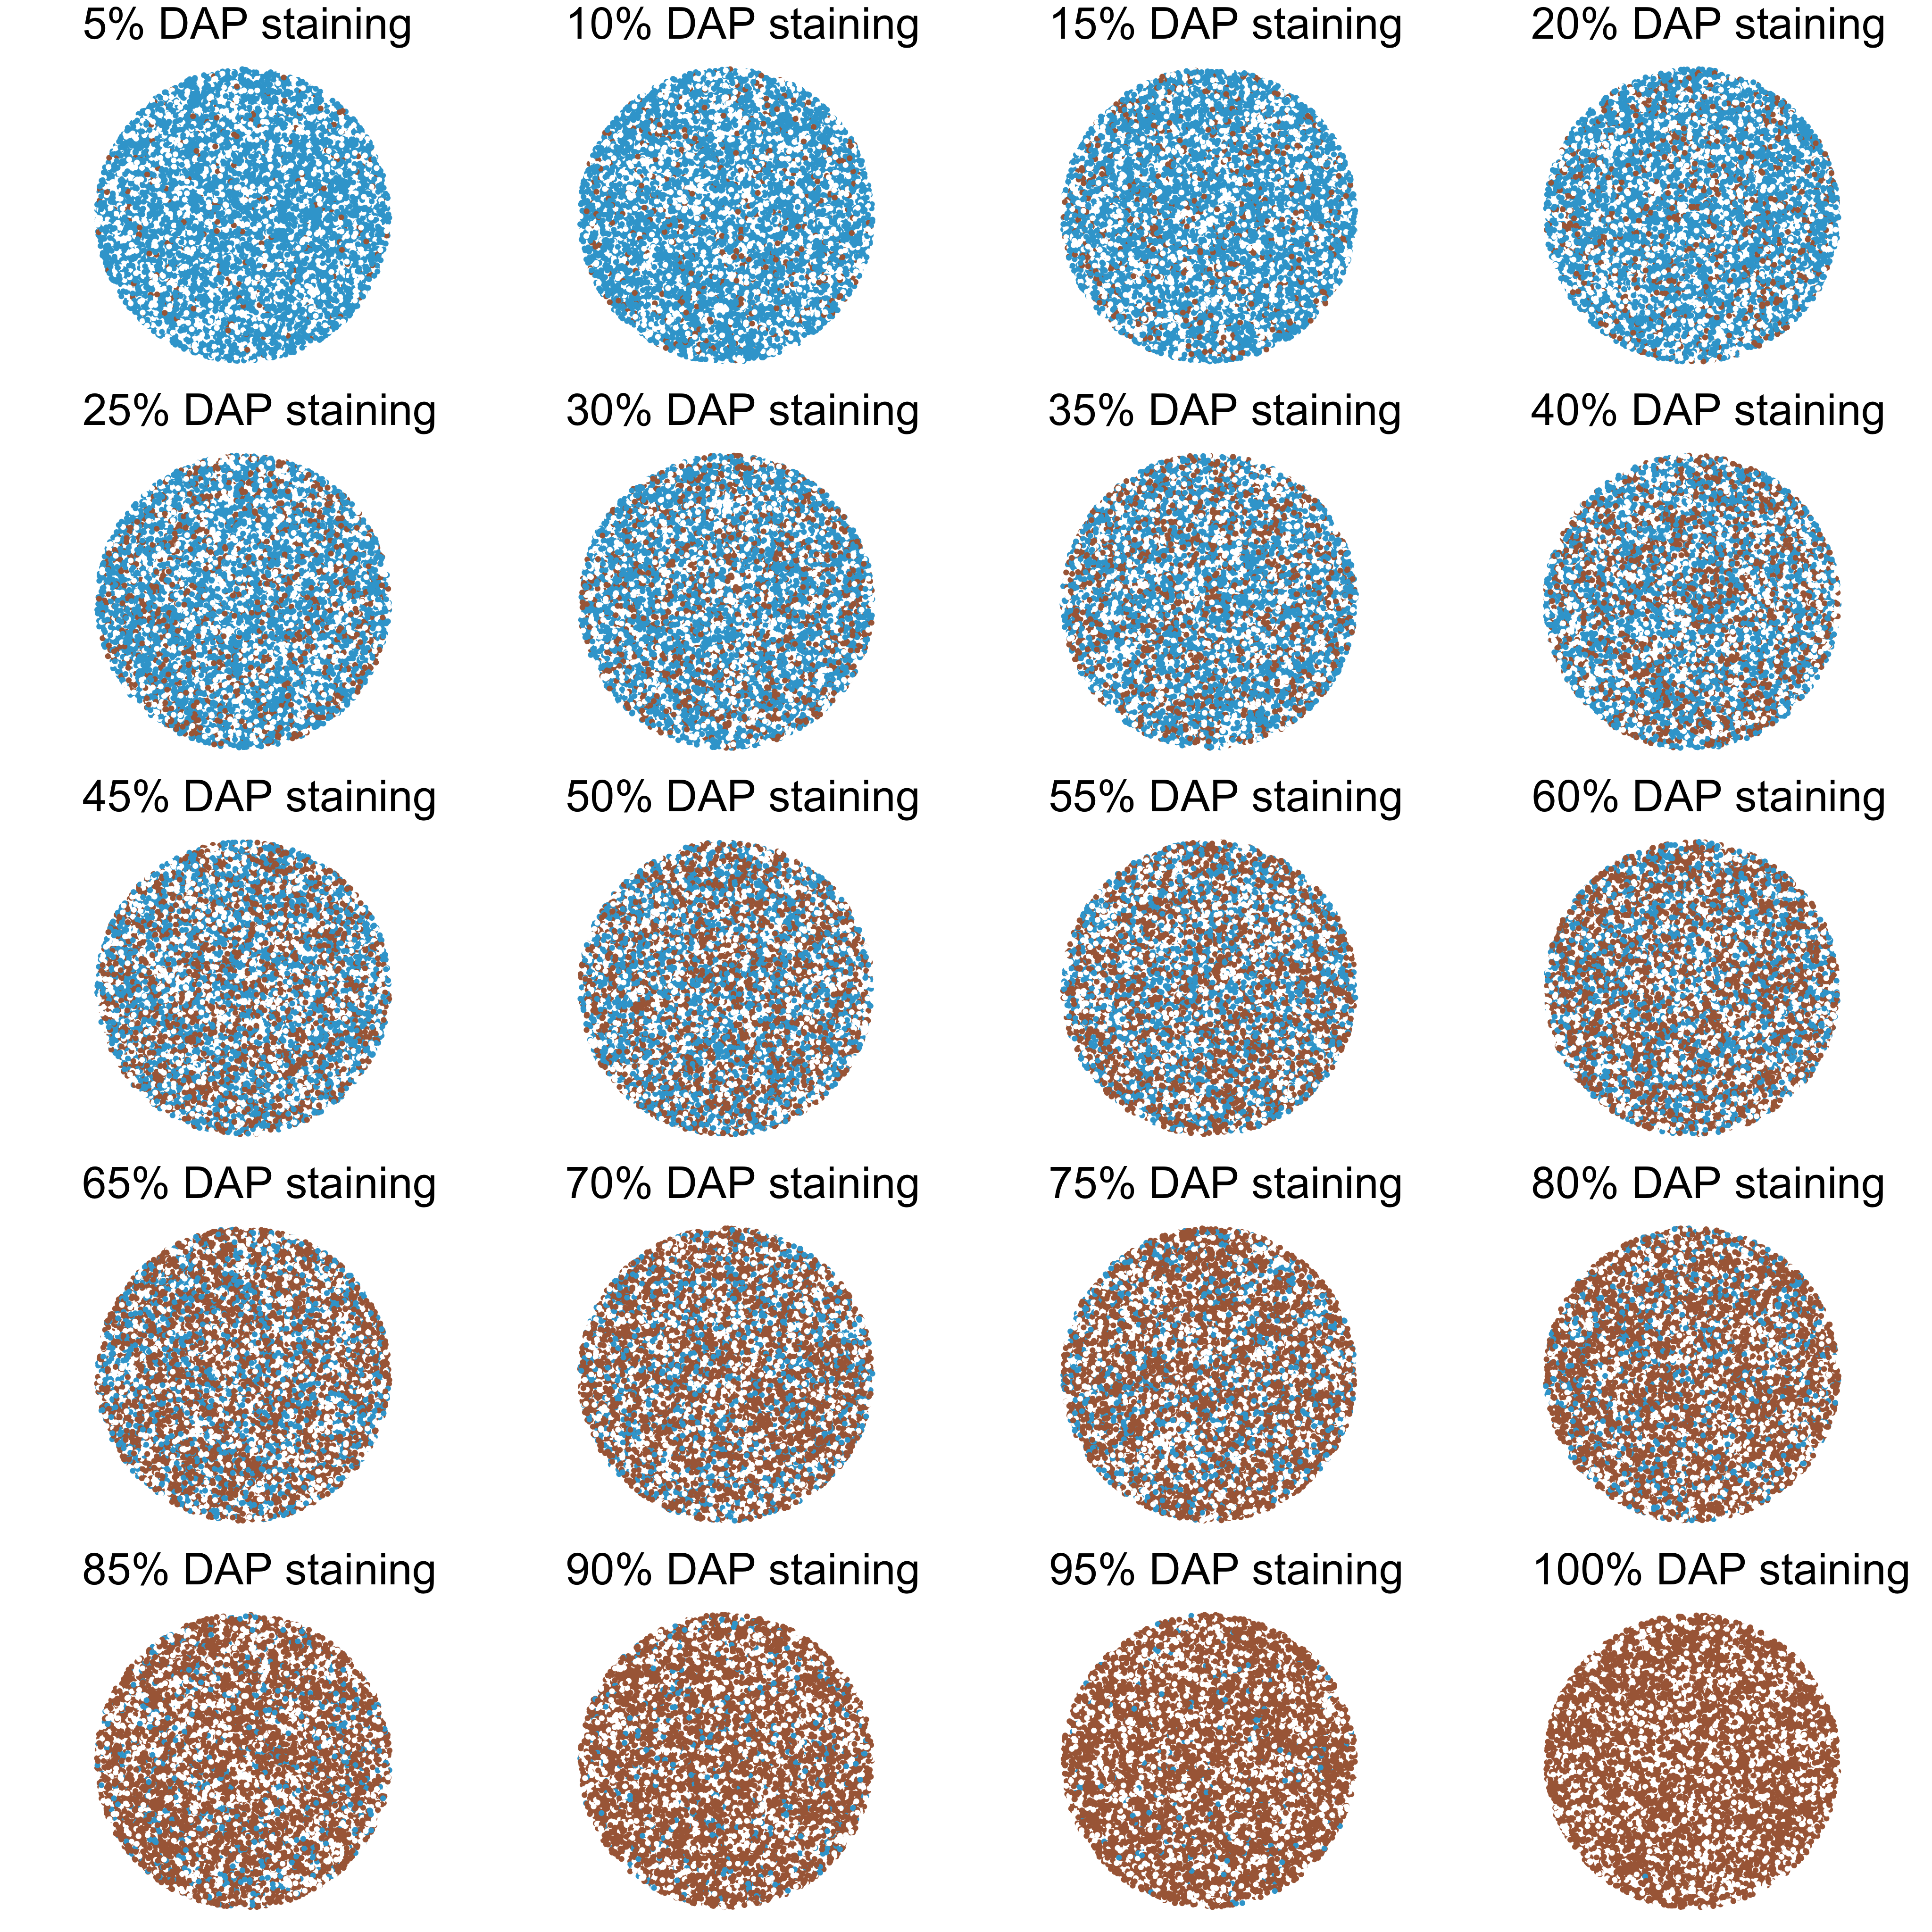
\includegraphics[width=0.7\linewidth]{2018-01-14-graphical-simulation-of-tissue-microarray-tma_files/figure-latex/unnamed-chunk-1-1}


\end{document}
